% ************ Anexo  ************
\renewcommand{\appendixname}{Anexo}
\appendix
\chapter{Documento com as alternativas para o desenvolvimento do projeto entregue à administração}
\label{anexo:A}

O documento a seguir foi produzido para informar a administração das diferentes opções tecnológicas para o desenvolvimento da plataforma solicitada pela empresa.

\newpage

\begin{figure}[H]
	\centering
	
\includegraphics[width=\linewidth, frame]{figuras/Alternativas/pag0.jpg}
	\caption{Capa do documento}
	\label{fig:anexo_a_capa}
\end{figure}
\newpage

\begin{figure}[H]
	\centering
	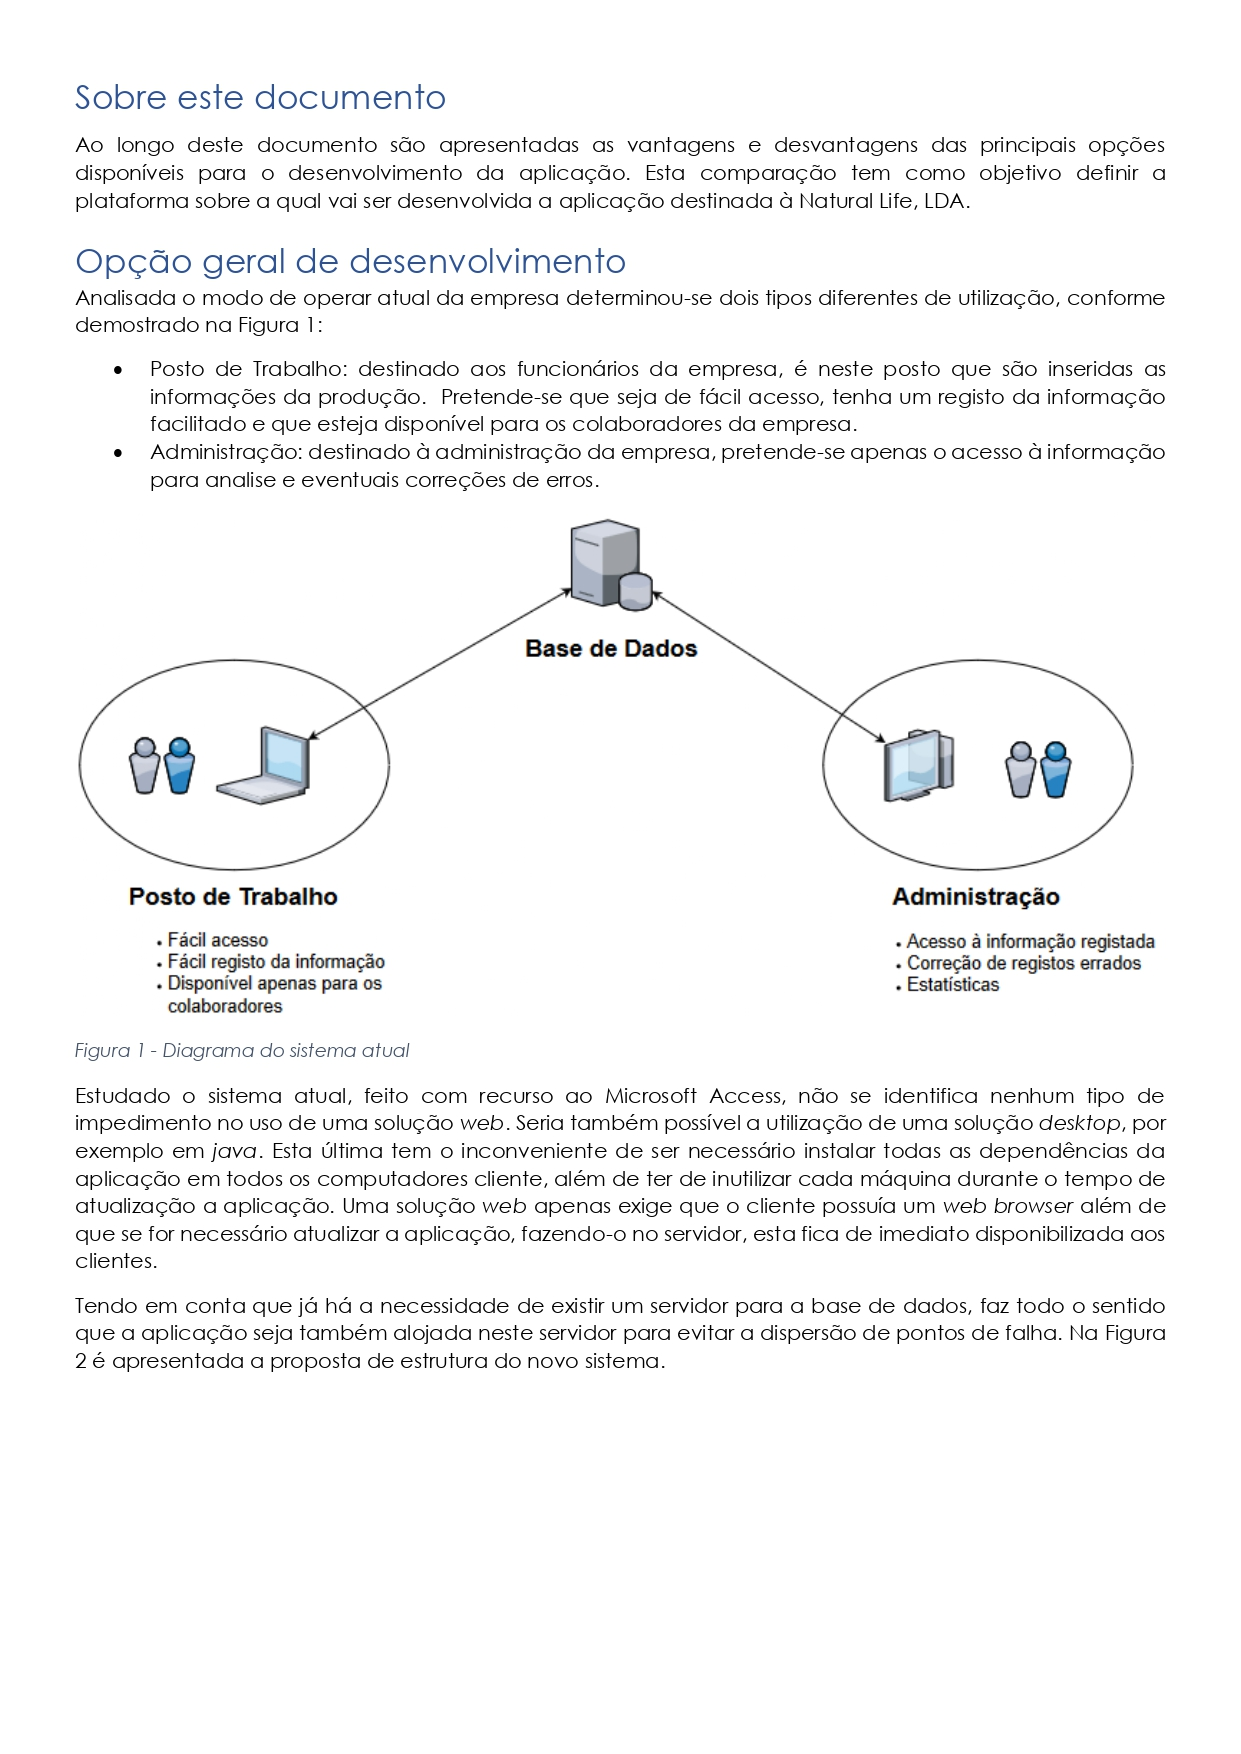
\includegraphics[width=\linewidth, frame]{figuras/Alternativas/pag1.jpg}
	\caption{Página 1}
	\label{fig:anexo_a_1}
\end{figure}
\newpage

\begin{figure}[H]
	\centering
	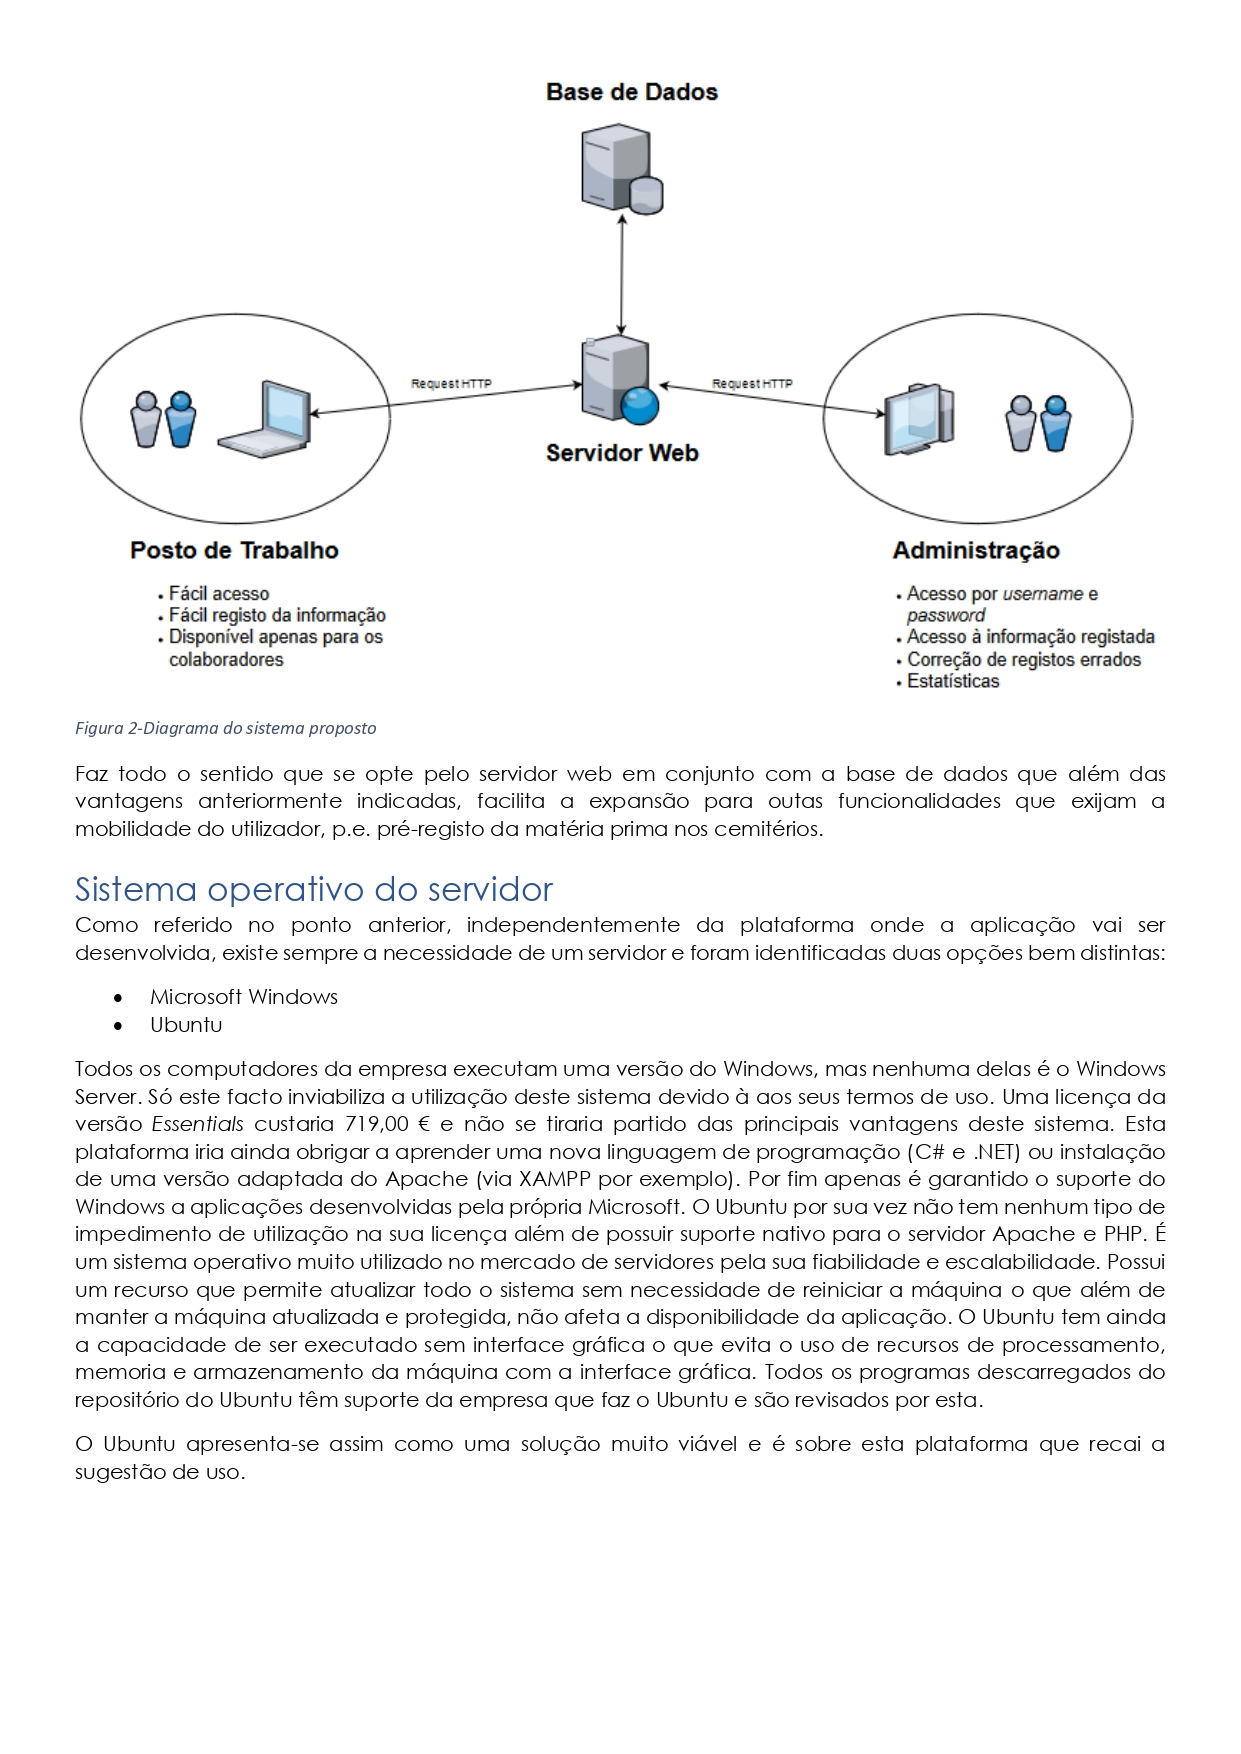
\includegraphics[width=\linewidth, frame]{figuras/Alternativas/pag2.jpg}
	\caption{Página 2}
	\label{fig:anexo_a_2}
\end{figure}
\newpage

\begin{figure}[H]
	\centering
	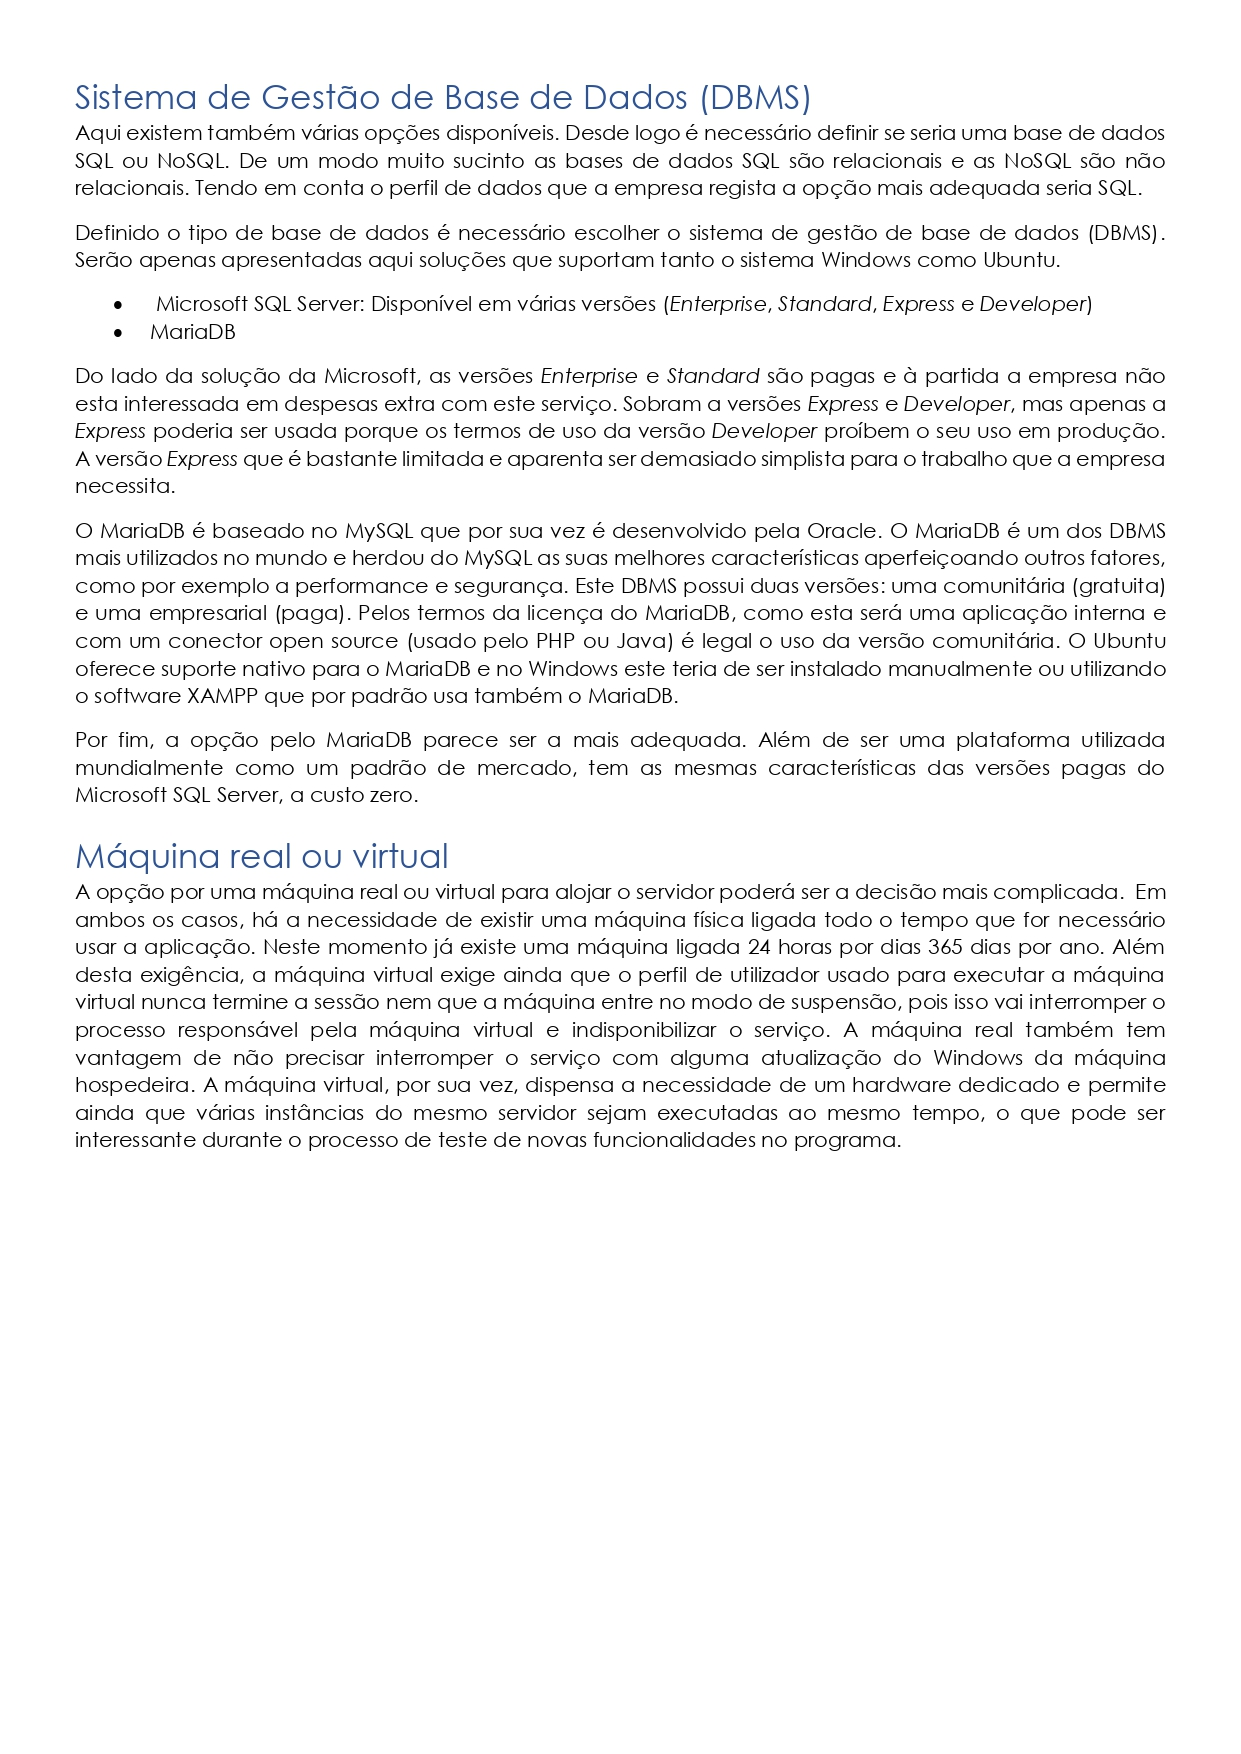
\includegraphics[width=\linewidth, frame]{figuras/Alternativas/pag3.jpg}
	\caption{Página 3}
	\label{fig:anexo_a_3}
\end{figure}
\newpage

\begin{figure}[H]
	\centering
	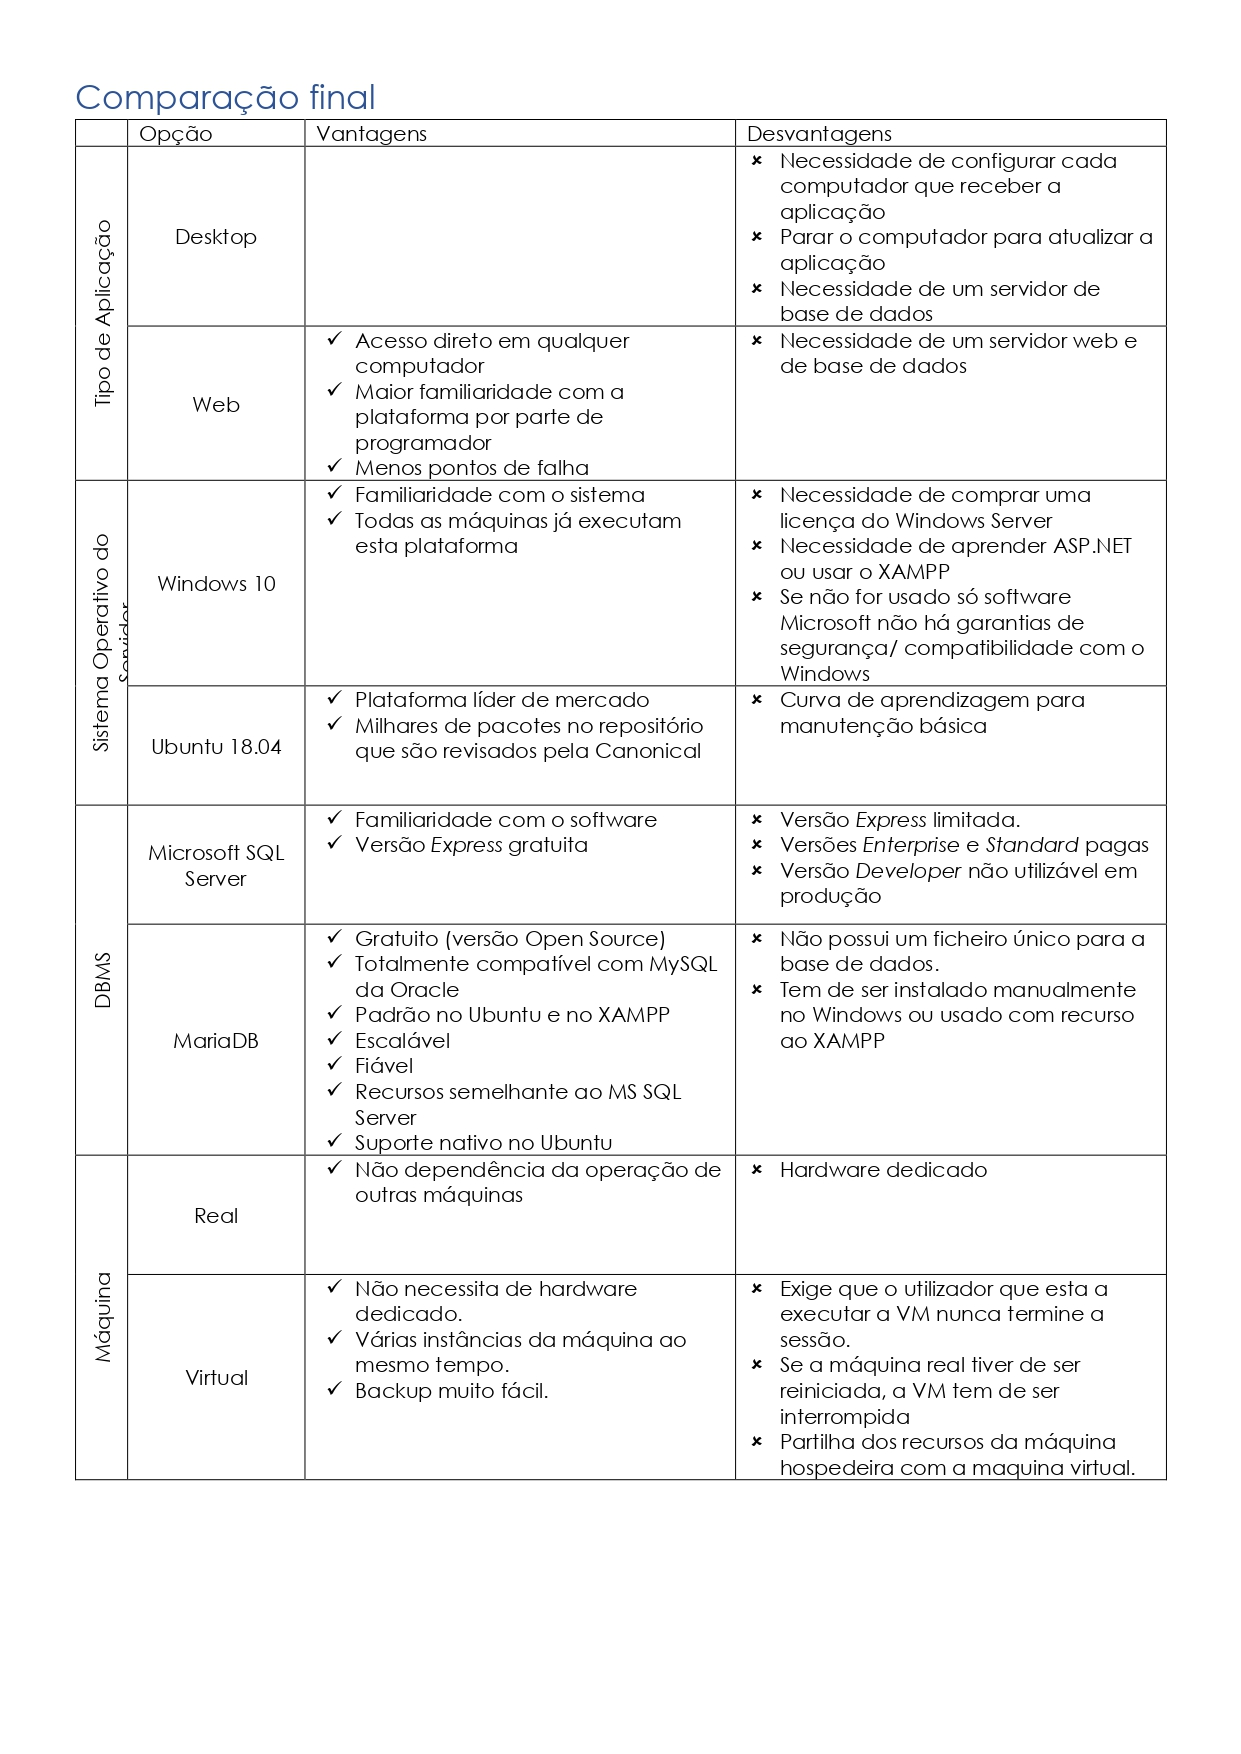
\includegraphics[width=\linewidth, frame]{figuras/Alternativas/pag4.jpg}
	\caption{Página 4}
	\label{fig:anexo_a_4}
\end{figure}
\newpage

\begin{figure}[H]
	\centering
	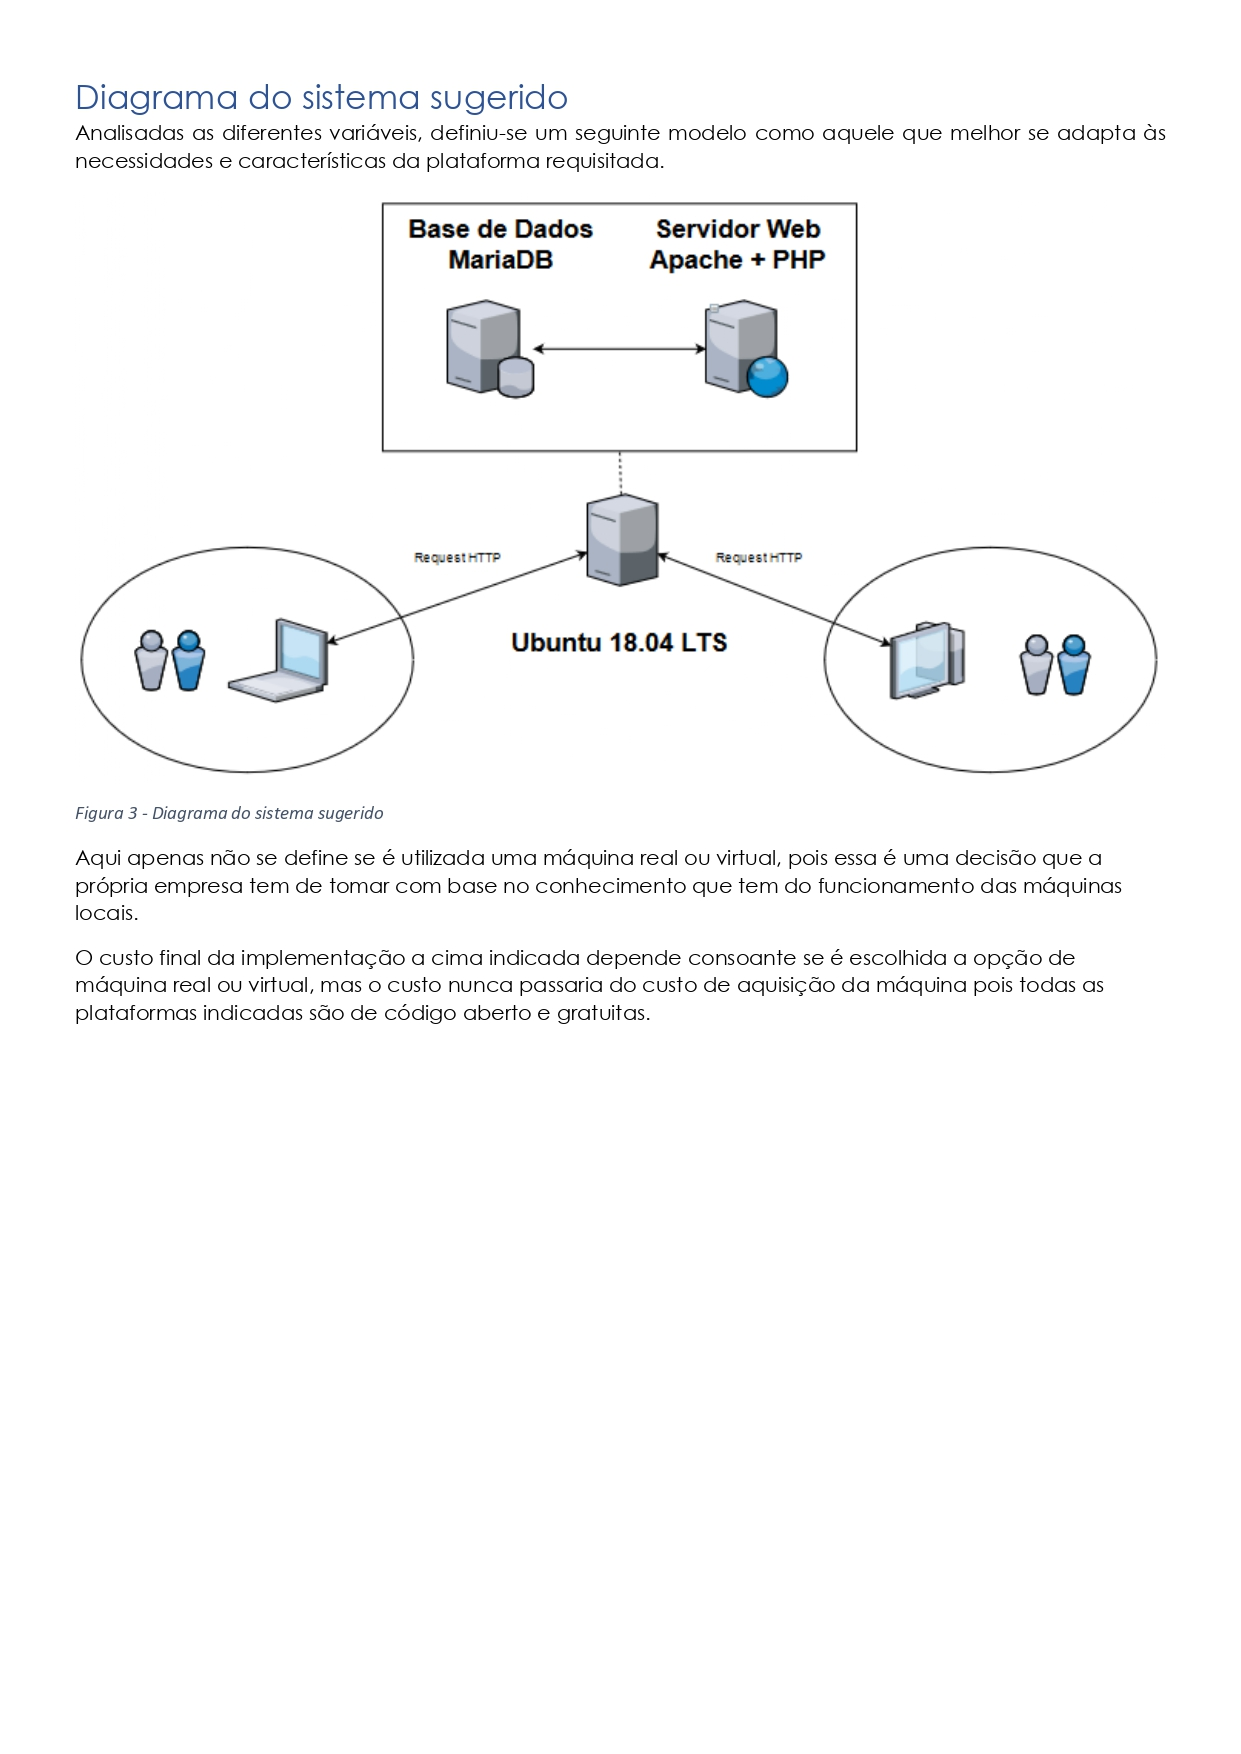
\includegraphics[width=\linewidth, frame]{figuras/Alternativas/pag5.jpg}
	\caption{Página 5}
	\label{fig:anexo_a_5}
\end{figure}